\begin{figure*}[ht!]
    \centering
    \RawFloats
    \begin{minipage}{0.65\textwidth}
    	\vspace{-20pt}
        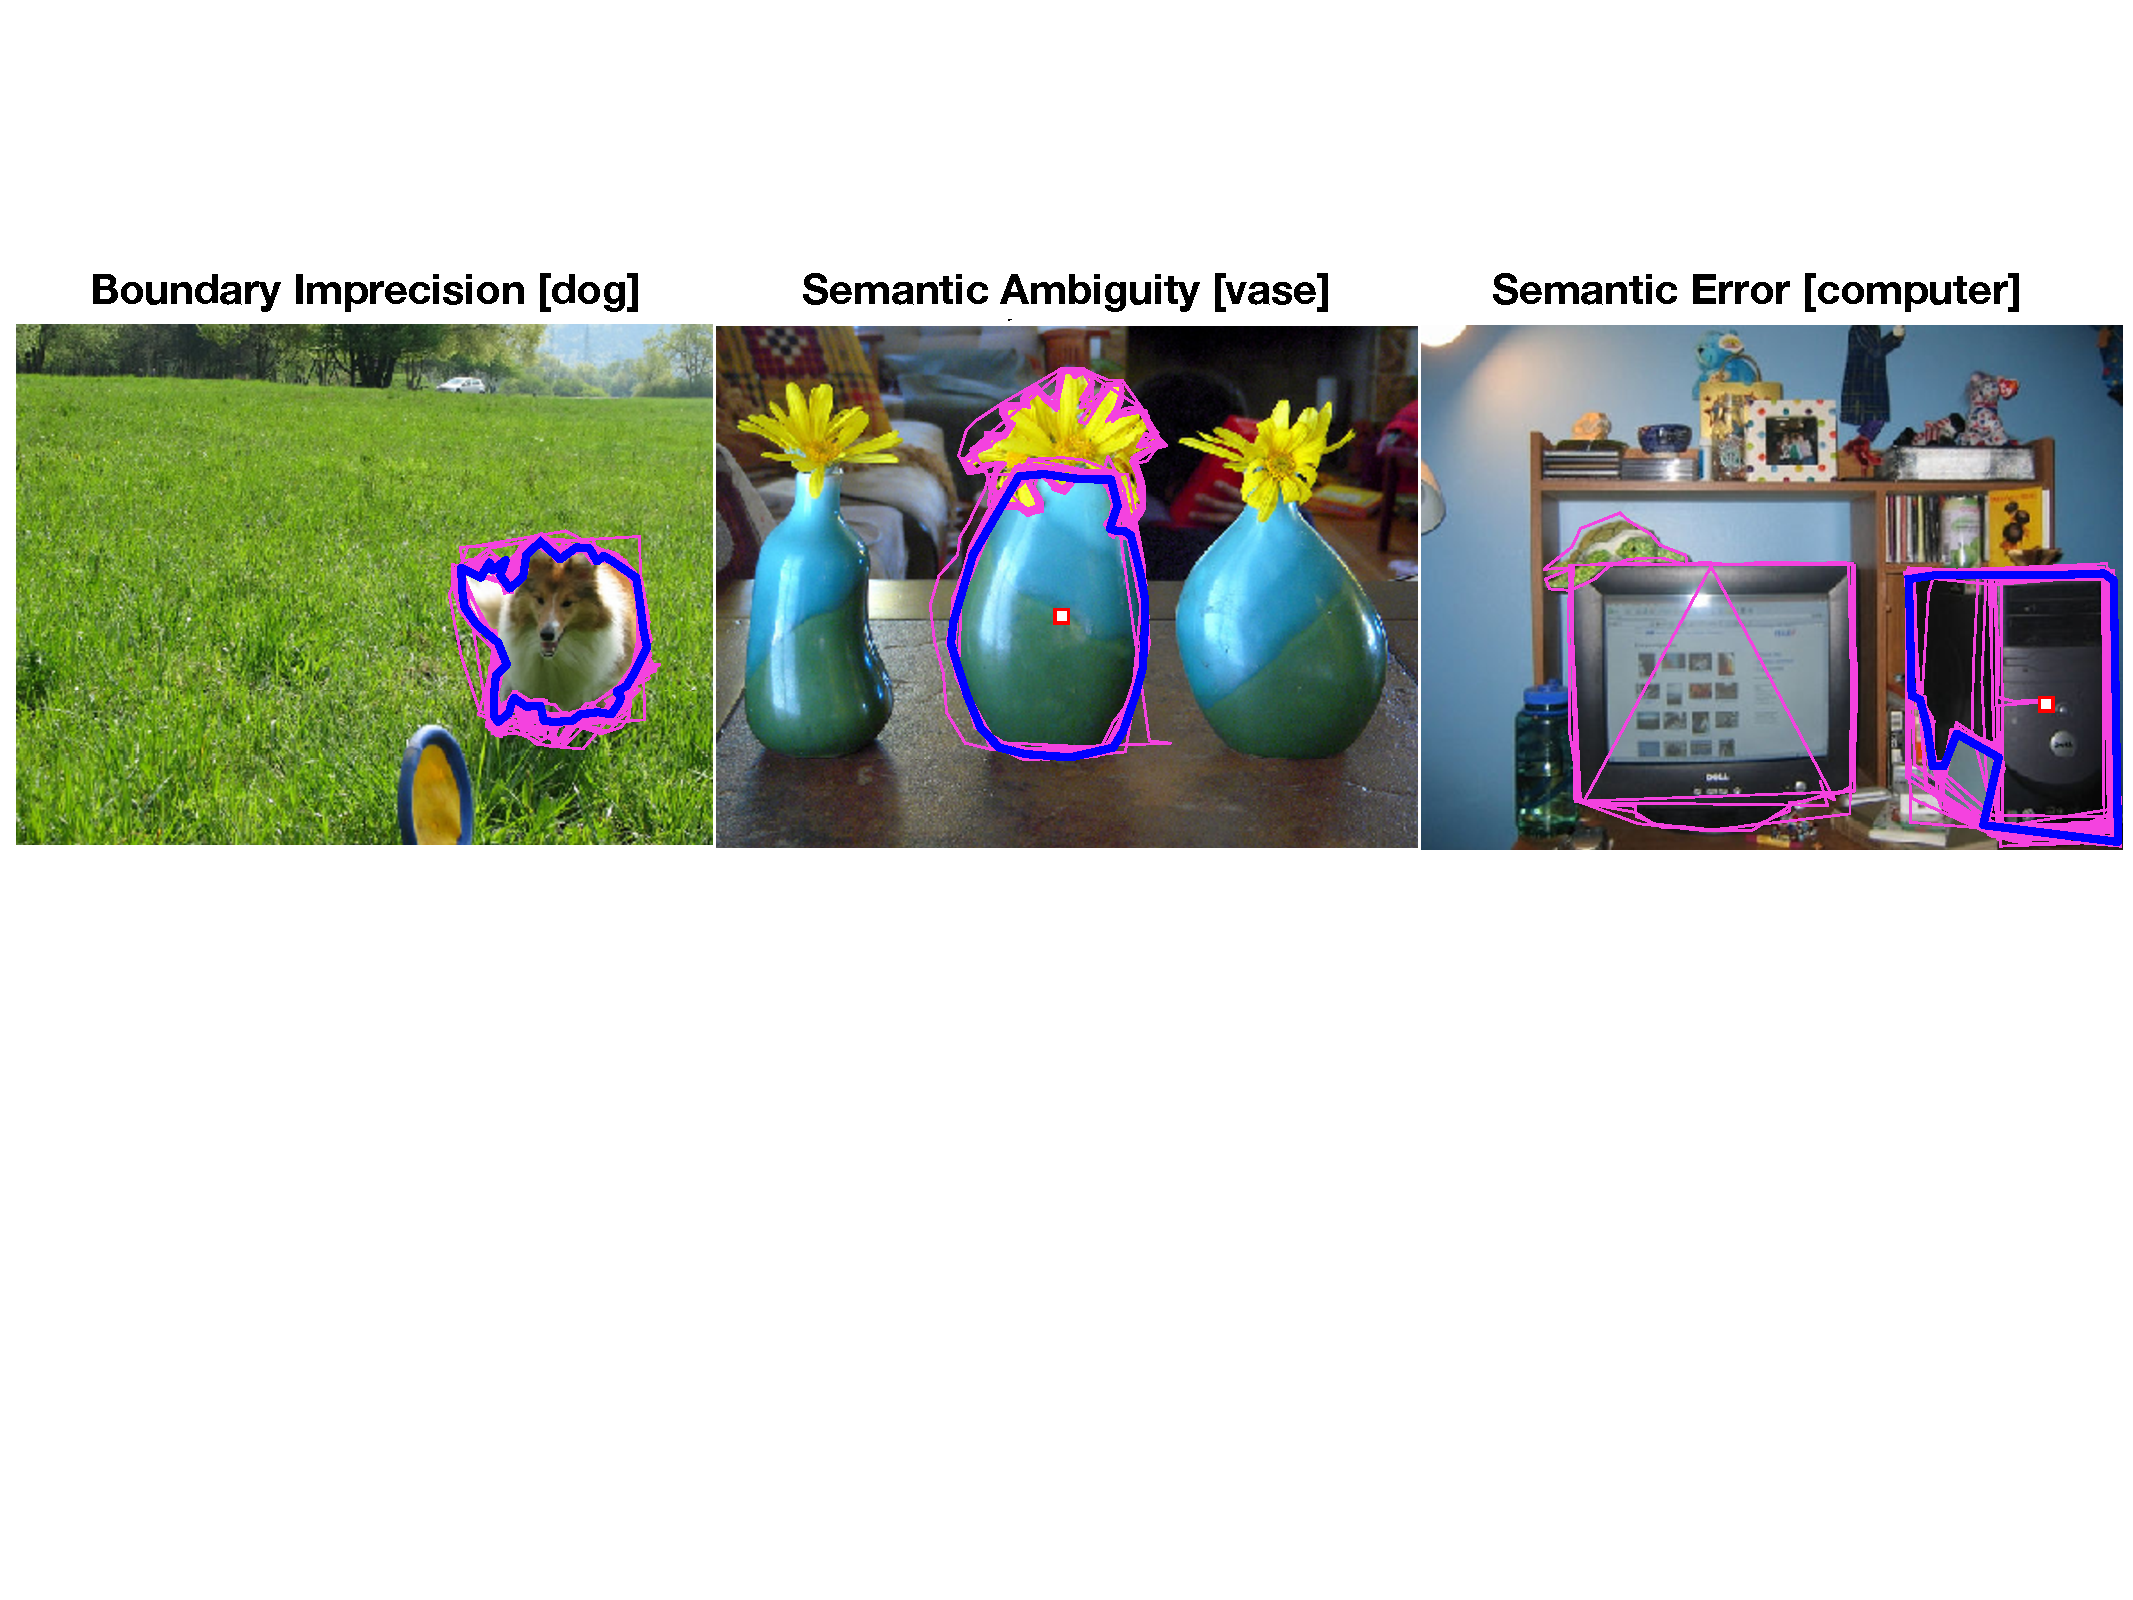
\includegraphics[width=\textwidth]{plots/error_examples.pdf} % second figure itself
        \caption{Pink is the segmentation from individual workers. Blue solid line delineates the ground truth. The red boxed pointer indicates the task of interest shown to users.}
        \vspace{-15pt}
        \label{error_examples}
    \end{minipage}
    \begin{minipage}{0.35\textwidth}
    	\vspace{-25pt}
        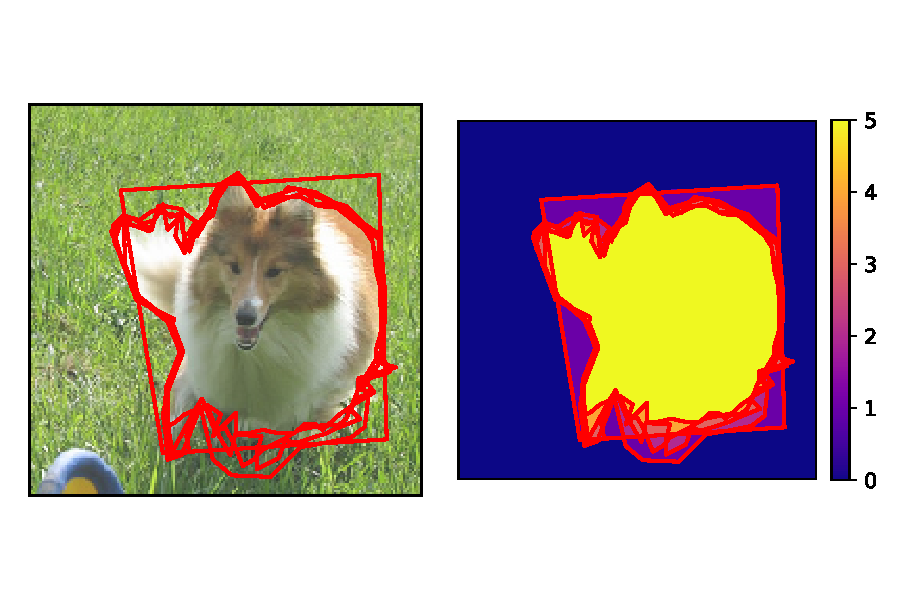
\includegraphics[width=\textwidth]{plots/tile_demo.pdf}
        \vspace{-35pt}
        \caption{Left: Segmentation boundaries drawn by five workers in red. Right: Overlaid segmentation creates a masks where the color indicates the number of workers who voted for the tile region.}
        \vspace{-20pt}
        \label{tile_demo}
    \end{minipage}\hfill
\end{figure*}
\section{Preliminaries}
\subsection{Data \& Goals}
We collected crowdsourced segmentation data from Amazon Mechanical Turk where each HIT consisted of one segmentation task for a specific pre-labeled object in the image. There were a total of 46 objects in 9 images from the MSCOCO dataset~\cite{Lin2014}. For each object, we collected segmentation masks from a total of 40 workers. Each task contains a semantic keyword and a pointer indicating the object to be segmented. These tasks represent a diverse set of task difficulty (different levels of clutteredness, occlusion, lighting) and levels of task ambiguity. %Given a raw 
\subsection{Evaluation Metrics}
\par Evaluation metrics used in our experiment measures how well the final segmentation (S) produced by these algorithms compare against ground truth (GT). The most common evaluation metric used in literature are area-based methods which take into account the intersection, $IA=area(S\cup GT)$, or union, $UA=area(S\cap GT)$, between the user and the ground truth segmentations. Specifically, we use
    $\text{Precision (P)} = \frac{IA(S)}{area(S)}$, 
    $\text{Recall (R)} = \frac{IA(S)}{area(GT)}$, and 
    $\text{Jaccard (J)} = \frac{UA(S)}{IA(S)}$
    metrics to evaluate our algorithms.
 \techreport{\par A sub-sampled dataset was created from the full dataset to determine the efficacy of these algorithms on varying number of worker responses. Every object was randomly sampled worker with replacement. For small worker samples, we average our results over larger number of batches than for large worker samples (which have lower variance, since the sample size is close to the original data size).}

\subsection{Error Analysis}
\par As shown in Figure \ref{error_examples} (left to right), common worker errors can be classified into three types: (1) \textbf{Boundary Imprecision:} unintentional mistakes while drawing the boundaries, either due to low precision of the image, small area of the object, or lack of drawing skills , (2) \textbf{Semantic Ambiguity:} have differing opinions about whether particular regions belong to part of an object; or (3) \textbf{Semantic Mistakes:} annotate the wrong object entirely.
\par %Out of the 46 objects in our dataset, 9 objects suffer from semantic ambiguity, 18 objects from semantic mistakes, and almost all objects suffer from some form of boundary imprecision to varying degrees. 
Since the main focus for quality evaluation in past literature have been focused on finding worker segmentation with minimal boundary precision issues, we will first describe novel aggregation-based algorithms that we have developed and compare them with existing retrieval-based methods for addressing boundary imprecision. In the following section, we will discuss a preprocessing method that we have developed to resolve the semantic ambiguity and mistakes, which have been observed in prior work~\cite{Sorokin2008,Lin2014,Gurari2018}.